\documentclass{article}




\usepackage{fullpage}
\usepackage{nopageno}
\usepackage{amsmath}
\usepackage{amsfonts}
\usepackage{graphicx}
\usepackage{framed}
\usepackage{algorithmic}
\usepackage{xcolor}

\definecolor{dark_red}{rgb}{0.5,0.0,0.0}
\definecolor{dark_green}{rgb}{0.0,0.5,0.0}
\definecolor{dark_blue}{rgb}{0.0,0.0,0.5}
\definecolor{blue}{rgb}{0.0,0.0,1.0}

\newcommand{\dr}[1]{\textcolor{dark_red}{#1}}
\newcommand{\dg}[1]{\textcolor{dark_green}{#1}}
\newcommand{\db}[1]{\textcolor{dark_blue}{#1}}
\newcommand{\blue}[1]{\textcolor{blue}{#1}}


\usepackage{fancyhdr}
%\setlength{\footheight}{15.2pt}
\pagestyle{fancy}
\fancyhead[C]{Wentworth Institute of Technology, MATH2025}
\fancyfoot[C]{Author: Shawn Eastwood}
\renewcommand{\headsep}{25pt}
\renewcommand{\headrulewidth}{1pt}
\renewcommand{\footrulewidth}{1pt}


\begin{document}

\section*{Quadratic surfaces}

Surfaces in 3D space are intrinsically represented by a single equation:
\[f(x, y, z) = g(x, y, z)\]

A {\bf quadratic surface} is a surface whose equation has the form:

\[Ax^2 + By^2 + Cz^2 + Dyz + Exz + Fyz + Gx + Hy + Iz = J\]

For this discussion, the coefficients of the mixed terms \(yz\), \(zx\), and \(xy\) will be set to \(0\):
\[D = E = F = 0\]
Also, at least \(2\) of \(A\), \(B\), and \(C\) will be nonzero. The quadratic surfaces will have equations of the form:

\[Ax^2 + By^2 + Cz^2 + Gx + Hy + Iz = J\]

%\[s_x\left(\frac{x - x_0}{r_x}\right)^2 + s_y\left(\frac{y - y_0}{r_y}\right)^2 + s_z\left(\frac{z - z_0}{r_z}\right)^2 = S\]
%where \(s_x\), \(s_y\), and \(s_z\) are chosen from the set \(\{-1, 0, 1\}\), and \(S\) is chosen from the set \(\{0, 1\}\).



\subsection*{Moving and stretching surfaces}

Given any arbitrary surface with the parametric equations:
\[\left\{\begin{array}{c} x(t_1, t_2) = h_x(t_1, t_2) \\ y(t_1, t_2) = h_y(t_1, t_2) \\ z(t_1, t_2) = h_z(t_1, t_2) \end{array}\right.\]

and the implicit equation:
\[f(x, y, z) = g(x, y, z)\]

\vspace{5mm}

Moving the surface through a displacement of \(\begin{bmatrix} x_0 \\ y_0 \\ z_0 \end{bmatrix}\), changes the parametric equations and the implicit equation respectively to:
\[\left\{\begin{array}{c} x(t_1, t_2) = h_x(t_1, t_2) + x_0 \\ y(t_1, t_2) = h_y(t_1, t_2) + y_0 \\ z(t_1, t_2) = h_z(t_1, t_2) + z_0 \end{array}\right.\]
and 
\[f(x - x_0, y - y_0, z - z_0) = g(x - x_0, y - y_0, z - z_0)\]

\vspace{5mm}

Stretching the surface parallel to the \(x\), \(y\), and \(z\) axes, by the respective factors \(r_x\), \(r_y\), and \(r_z\), changes the parametric equations and the implicit equation respectively to:
\[\left\{\begin{array}{c} x(t_1, t_2) = r_x h_x(t_1, t_2) \\ y(t_1, t_2) = r_y h_y(t_1, t_2) \\ z(t_1, t_2) = r_z h_z(t_1, t_2) \end{array}\right.\]
and 
\[f(x/r_x, y/r_y, z/r_z) = g(x/r_x, y/r_y, z/r_z)\]

\vspace{5mm}

Now stretch the surface parallel to the \(x\), \(y\), and \(z\) axes, by the respective factors \(r_x\), \(r_y\), and \(r_z\), and then move the surface through a displacement of \(\begin{bmatrix} x_0 \\ y_0 \\ z_0 \end{bmatrix}\). The parametric equations and the implicit equation are respectively changed to:
\[\left\{\begin{array}{c} x(t_1, t_2) = r_x h_x(t_1, t_2) + x_0 \\ y(t_1, t_2) = r_y h_y(t_1, t_2) + y_0 \\ z(t_1, t_2) = r_z h_z(t_1, t_2) + z_0 \end{array}\right.\]
and 
\[f\left(\frac{x - x_0}{r_x}, \frac{y - y_0}{r_y}, \frac{z - z_0}{r_z}\right) = g\left(\frac{x - x_0}{r_x}, \frac{y - y_0}{r_y}, \frac{z - z_0}{r_z}\right)\]


The following sections will examine each ``type" of quadratic surface. The ``default" equation for each surface will be given, but always remember that the general equation results from replacing \(x\) with \(\frac{x - x_0}{r_x}\), \(y\) with \(\frac{y - y_0}{r_y}\), and \(z\) with \(\frac{z - z_0}{r_z}\). 


\subsection*{All quadratic coefficients are nonzero}

The first quadratic surfaces that will be analyzed will be those for which the coefficients of \(x^2\), \(y^2\), and \(z^2\) are all nonzero.

\subsubsection*{Ellipsoids} 

\begin{tabular}{cc}
\parbox{0.5\textwidth}{
To the right, a graph of the equation 
\[x^2 + y^2 + z^2 = 1\]
is shown. This is a unit sphere centered on the origin. Stretching the surface parallel to the \(x\), \(y\), and \(z\) axes by the respective factors \(r_x\), \(r_y\), and \(r_z\), and then moving the surface through a displacement of \(\begin{bmatrix} x_0 \\ y_0 \\ z_0 \end{bmatrix}\) yields an {\bf ellipsoid}.
\[\left(\frac{x - x_0}{r_x}\right)^2 + \left(\frac{y - y_0}{r_y}\right)^2 + \left(\frac{z - z_0}{r_z}\right)^2 = 1\]    
} & \parbox{0.5\textwidth}{
\includegraphics[width = 0.5\textwidth]{ellipsoid.png}
}
\end{tabular}

\subsubsection*{Hyperboloids with 1 sheet} 

\begin{tabular}{cc}
\parbox{0.5\textwidth}{
To the right, a graph of the equation 
\[x^2 + y^2 - z^2 = 1\]
is shown. This is a {\bf hyperboloid with 1 sheet} oriented along the \(z\)-axis. The hyperboloid can be oriented along the other axes as well. The ``default" equations for the hyperboloid with 1 sheet are: \\
Along the \(x\)-axis:
\[-x^2 + y^2 + z^2 = 1\]
Along the \(y\)-axis:
\[x^2 - y^2 + z^2 = 1\]
Along the \(z\)-axis:
\[x^2 + y^2 - z^2 = 1\]
} & \parbox{0.5\textwidth}{
\includegraphics[width = 0.5\textwidth]{1_sheet_hyperboloid.png}
}
\end{tabular}

\subsubsection*{Hyperboloids with 2 sheets} 

\begin{tabular}{cc}
\parbox{0.5\textwidth}{
To the right, a graph of the equation 
\[-x^2 - y^2 + z^2 = 1\]
is shown. This is a {\bf hyperboloid with 2 sheets} oriented along the \(z\)-axis. The hyperboloid can be oriented along the other axes as well. The ``default" equations for the hyperboloid with 2 sheets are: \\
Along the \(x\)-axis:
\[x^2 - y^2 - z^2 = 1\]
Along the \(y\)-axis:
\[-x^2 + y^2 - z^2 = 1\]
Along the \(z\)-axis:
\[-z^2 - y^2 + z^2 = 1\]
} & \parbox{0.5\textwidth}{
\includegraphics[width = 0.5\textwidth]{2_sheet_hyperboloid.png}
}
\end{tabular}




\subsubsection*{Nothing}

The equation 
\[-x^2 - y^2 - z^2 = 1\]
is never true for all real values of \(x\), \(y\), and \(z\).


\subsubsection*{A single point}

The equation 
\[x^2 + y^2 + z^2 = 0\]
is true only for \((x, y, z) = (0, 0, 0)\).



\subsubsection*{Cones}

\begin{tabular}{cc}
\parbox{0.5\textwidth}{
To the right, a graph of the equation 
\[x^2 + y^2 - z^2 = 0\]
is shown. This is a {\bf double cone} oriented along the \(z\)-axis. The double cone can be oriented along the other axes as well. The ``default" equations for the double cone are: \\
Along the \(x\)-axis:
\[-x^2 + y^2 + z^2 = 0\]
Along the \(y\)-axis:
\[x^2 - y^2 + z^2 = 0\]
Along the \(z\)-axis:
\[x^2 + y^2 - z^2 = 0\]
} & \parbox{0.5\textwidth}{
\includegraphics[width = 0.5\textwidth]{cones.png}
}
\end{tabular}



\subsection*{1 quadratic coefficient is 0}

Now, quadratic surfaces where exactly one of the coefficients of \(x^2\), \(y^2\), and \(z^2\) is \(0\) will be analyzed.


\subsubsection*{Elliptic Paraboloids}

\begin{tabular}{cc}
\parbox{0.5\textwidth}{
To the right, a graph of the equation 
\[z = x^2 + y^2\]
is shown. This is an {\bf elliptic paraboloid} oriented along the \(z\)-axis. The elliptic paraboloid can be oriented along the other axes as well. The ``default" equations for the elliptic paraboloid are: \\
Along the \(x\)-axis:
\[x = \pm y^2 \pm z^2\]
Along the \(y\)-axis:
\[y = \pm x^2 \pm z^2\]
Along the \(z\)-axis:
\[z = \pm x^2 \pm y^2\]
} & \parbox{0.5\textwidth}{
\includegraphics[width = 0.5\textwidth]{elliptic_paraboloid.png}
}
\end{tabular}




\subsubsection*{Hyperbolic paraboloids}

\begin{tabular}{cc}
\parbox{0.5\textwidth}{
To the right, a graph of the equation 
\[z = x^2 - y^2\]
is shown. This is a {\bf hyperbolic paraboloid} oriented along the \(z\)-axis. The hyperbolic paraboloid can be oriented along the other axes as well. The ``default" equations for the hyperbolic paraboloid are: \\
Along the \(x\)-axis:
\[x = \pm y^2 \mp z^2\]
Along the \(y\)-axis:
\[y = \pm x^2 \mp z^2\]
Along the \(z\)-axis:
\[z = \pm x^2 \mp y^2\]
} & \parbox{0.5\textwidth}{
\includegraphics[width = 0.5\textwidth]{hyperbolic_paraboloid.png}
}
\end{tabular}



\subsubsection*{Elliptic Cylinders} 

\begin{tabular}{cc}
\parbox{0.5\textwidth}{
To the right, a graph of the equation 
\[x^2 + y^2 = 1\]
is shown. This is an {\bf elliptic cylinder} oriented along the \(z\)-axis. The elliptic cylinder can be oriented along the other axes as well. The ``default" equations for the elliptic cylinder are: \\ 
Along the \(x\)-axis:
\[y^2 + z^2 = 1\]
Along the \(y\)-axis:
\[x^2 + z^2 = 1\]
Along the \(z\)-axis:
\[x^2 + y^2 = 1\]
} & \parbox{0.5\textwidth}{
\includegraphics[width = 0.5\textwidth]{elliptic_cylinder.png}
}
\end{tabular}




\subsubsection*{Hyperbolic Cylinders} 

\begin{tabular}{cc}
\parbox{0.5\textwidth}{
To the right, a graph of the equation 
\[x^2 - y^2 = 1\]
is shown. This is a {\bf hyperbolic cylinder} oriented along the \(z\)-axis. The hyperbolic cylinder can be oriented along the other axes as well. The ``default" equations for the hyperbolic cylinder are: \\ 
Along the \(x\)-axis:
\[\pm y^2 \mp z^2 = 1\]
Along the \(y\)-axis:
\[\pm x^2 \mp z^2 = 1\]
Along the \(z\)-axis:
\[\pm x^2 \mp y^2 = 1\]
} & \parbox{0.5\textwidth}{
\includegraphics[width = 0.5\textwidth]{hyperbolic_cylinder.png}
}
\end{tabular}




\subsection*{Identifying surfaces}

Given an equation of the form
\[Ax^2 + By^2 + Cz^2 + Gx + Hy + Iz = J\]
how can the surface be identified?

The first step is to count how many of \(x^2\), \(y^2\), and \(z^2\) have nonzero coefficients. At least 2 of \(x^2\), \(y^2\), and \(z^2\) will have nonzero coefficients.
\begin{itemize}
	\item If all of \(x^2\), \(y^2\), and \(z^2\) have nonzero coefficients, then the surface is either an ellipsoid; hyperboloid with 1 sheet; hyperboloid with 2 sheets; nothing; a single point; or a double cone. Complete the square for each variable to get an equation with the form:
	\[A(x - x_0)^2 + B(y - y_0)^2 + C(z - z_0)^2 = K\]
	Since completing the square involves the addition of constant terms, \(K \neq J\) in most cases. 
	\begin{itemize}
		\item[*] If \(K \neq 0\), then divide both sides by \(K\) to get a \(1\) on the right hand side:
		\[(A/K)(x - x_0)^2 + (B/K)(y - y_0)^2 + (C/K)(z - z_0)^2 = 1\]
		Rewrite the equation to get:
		\[\pm\left(\frac{x - x_0}{r_x}\right)^2 \pm \left(\frac{y - y_0}{r_y}\right)^2 \pm\left(\frac{z - z_0}{r_z}\right)^2 = 1\]
		where \(r_x = \sqrt{|K/A|}\), \(r_y = \sqrt{|K/B|}\), and \(r_z = \sqrt{|K/C|}\). \\
		The surface can easily identified by the sign of each component in the sum. \(3\) positives means an ellipsoid, \(2\) positives means a hyperboloid with 1 sheet, \(1\) positive means a hyperboloid with 2 sheets, and \(0\) positives means nothing.
		\item[*] If \(K = 0\), then multiply both sides by \(+1\) or \(-1\) so a majority of the coefficients \(A\), \(B\), and \(C\) become positive. Rewrite the equation to get:
		\[\pm\left(\frac{x - x_0}{r_x}\right)^2 \pm \left(\frac{y - y_0}{r_y}\right)^2 \pm\left(\frac{z - z_0}{r_z}\right)^2 = 0\] 
		where \(r_x = 1/\sqrt{|A|}\), \(r_y = 1/\sqrt{|B|}\), and \(r_z = 1/\sqrt{|C|}\). \\
		The surface can easily identified by the sign of each component in the sum. \(3\) positives means a point, and \(2\) positives means a double cone.
	\end{itemize}
	\item If two of \(x^2\), \(y^2\), and \(z^2\) have nonzero coefficients, then the surface is either an elliptic paraboloid; hyperbolic paraboloid; elliptic cylinder; hyperbolic cylinder; or some other undiscussed case.   
	\begin{itemize}
		\item[*] If the non-quadratic variable is still part of the equation, then express this variable as a function of the other 2 variables while completing the square with the other 2 variables. For example, if \(z\) is the non-quadratic variable, but is still present in the equation, then rewrite the equation to get:
		\[z = z_0 + a(x - x_0)^2 + b(y - y_0)^2\]
		If \(a\) and \(b\) have the same sign, then the surface is an elliptic paraboloid, otherwise the surface is a hyperbolic paraboloid.
		\item[*] If the non-quadratic variable is completely absent from the equation, then complete the square with the other 2 variables. For example, if \(z\) is the non-quadratic variable, and is absent from the equation, then rewrite the equation to get:
		\[A(x - x_0)^2 + B(y - y_0)^2 = K\]
	\end{itemize}
\end{itemize}


\textbf{Examples:}
\begin{itemize}
%%%%%%%%%%%%%%%%%%%%%%%%
\item Consider the quadratic surface defined by:
\[x^2 + 9y^2 + 36z^2 - 4x + 18y + 216z = -328\]
what surface is this? Firstly, note that all of \(x^2\), \(y^2\), and \(z^2\) are present in the equation. Now complete the square for each variable:
\begin{align*}
& x^2 + 9y^2 + 36z^2 - 4x + 18y + 216z = -328 \\
\iff & (x^2 + 2(-2)x + (-2)^2) + 9(y^2 + 2(1)y + 1^2) + 36(z^2 + 2(3)z + 3^2) = -328 + (-2)^2 + 9(1^2) + 36(3^2) \\
\iff & (x - 2)^2 + 9(y + 1)^2 + 36(z + 3)^2 = 9 
\iff \left(\frac{x - 2}{3}\right)^2 + (y + 1)^2 + \left(\frac{z + 3}{1/2}\right)^2 = 1
\end{align*}   
This surface is an ellipsoid centered on the point \((x_0, y_0, z_0) = (2, -1, -3)\) with \(x\), \(y\), and \(z\) radii of \(r_x = 3\), \(r_y = 1\), and \(r_z = \frac{1}{2}\) respectively.
%%%%%%%%%%%%%%%%%%%%%%%%
\item Consider the quadratic surface defined by:
\[25x^2 - y^2 + 25z^2 + 50x - 100z = -100\]
what surface is this? Firstly, note that all of \(x^2\), \(y^2\), and \(z^2\) are present in the equation. Now complete the square for each variable:
\begin{align*}
& 25x^2 - y^2 + 25z^2 + 50x - 100z = -100 \\ 
\iff & 25(x^2 + 2(1)x + 1^2) - y^2 + 25(z^2 + 2(-2)z + (-2)^2) = -100 + 25(1^2) + 25(-2)^2 \\
\iff & 25(x + 1)^2 - y^2 + 25(z - 2)^2 = 25 \\   
\iff & (x + 1)^2 - \left(\frac{y}{5}\right)^2 + (z - 2)^2 = 1 
\end{align*}
This surface is a hyperboloid with 1 sheet, oriented along the \(y\)-axis, and centered on the point \((-1, 0, 2)\) with \(x\), \(y\), and \(z\) stretch factors of \(r_x = 1\), \(r_y = 5\), and \(r_z = 1\). 
%%%%%%%%%%%%%%%%%%%%%%%%
\item Consider the quadratic surface defined by:
\[y^2 + 4z^2 - 4x - 2y + 24z = -41\]  
what surface is this? Firstly, note that \(x^2\) is absent from the equation. \(x\) however, is still present in the equation, so solve the equation for \(x\): 
\begin{align*}
& y^2 + 4z^2 - 4x - 2y + 24z = -41  
\iff -4x = -41 - y^2 - 4z^2 + 2y - 24z \\
& \iff x = \frac{41}{4} + \frac{1}{4}y^2 + z^2 - \frac{1}{2}y + 6z
\end{align*}  
Now complete the square for variables \(y\) and \(z\):   
\begin{align*}
x = & \frac{41}{4} + \frac{1}{4}y^2 + z^2 - \frac{1}{2}y + 6z 
= \frac{41}{4} + \frac{1}{4}(y^2 + 2(-1)y + (-1)^2) + (z^2 + 2(3)z + 3^2) - \frac{1}{4}(-1)^2 - 3^2 \\
= & 1 + \frac{1}{4}(y - 1)^2 + (z + 3)^2
\end{align*}
This surface is a paraboloid, oriented along the \(x\)-axis, and centered on the point \((1, 1, -3)\). 
\end{itemize}




\section*{Calculus of parametric curves}

This section will cover vector valued functions. The input will be a single scalar (1 input), and the output will be a 3-component vector (3 outputs). 

Below is an example of a vector valued function:
\[\mathbf{q}(t) = \begin{bmatrix} 4t \\ -3t^2 + \sin(t) \\ 1/(1 + t^2) \end{bmatrix}\]
In this example \(\mathbf{q}(1) = \begin{bmatrix} 4(1) \\ -3(1)^2 + \sin(1) \\ 1/(1 + 1^2) \end{bmatrix} = \begin{bmatrix} 4 \\ -3 + \sin(1) \\ 1/2 \end{bmatrix}\), and \\ \(\mathbf{q}(-2) = \begin{bmatrix} 4(-2) \\ -3(-2)^2 + \sin(-2) \\ 1/(1 + (-2)^2) \end{bmatrix} = \begin{bmatrix} -8 \\ -12 - \sin(2) \\ 1/5 \end{bmatrix}\).


The domain of a vector valued function is the intersection of the domains of each of the functions for its 3 components. An arbitrary value \(t\) is part of the domain if and only if it is part of the domain of each of the 3 components. Consider for example the function:
\[\mathbf{q}(t) = \begin{bmatrix} \sqrt{t + 2} \\ 1/(t - 3) \\ 1/t \end{bmatrix}\]
The domain of the functions for each of the components (using interval notation) are: the first component has the domain \([-2, +\infty)\); the second component has the domain \((-\infty, 3) \cup (3, +\infty)\); and the third component has the domain \((-\infty, 0) \cup (0, +\infty)\). The intersection of these 3 domains is:
\[[-2, 0) \cup (0, 3) \cup (3, +\infty)\]




\subsection*{Limits}

The formal definition of the limit of a vector valued function will now be given. Given an arbitrary vector valued function \(\mathbf{q}(t)\), a scalar \(t_0\), and a vector \(\mathbf{p}\), then 
\[\mathbf{p} = \lim_{t \rightarrow t_0} \mathbf{q}(t)\]
if and only if for every strictly positive value of \(\epsilon\) (i.e. \(\epsilon > 0\)) there exists another strictly positive value \(\delta\) (i.e. \(\delta > 0\)) such that the following is true: \\ 
For any choice of {\bf non zero} \(h\) that is strictly within \(\delta\) of \(0\) (i.e. \(0 < |h| < \delta\)), the value of \(\mathbf{q}(t_0 + h)\) is also strictly within \(\epsilon\) of \(\mathbf{p}\) (i.e. \(\|\mathbf{q}(t_0 + h) - \mathbf{p}\| < \epsilon\). In essence,

\[0 < |h| < \delta \implies \|\mathbf{q}(t_0 + h) - \mathbf{p}\| < \epsilon\]

In summary, \(\mathbf{q}(t)\) must be ``close" to \(\mathbf{p}\) when \(t\) is ``close" to \(t_0\).

The limit of a vector valued function can be computed by computing the limits of each of its components.

\[\lim_{t \rightarrow t_0} \begin{bmatrix} f_x(t) \\ f_y(t) \\ f_z(t) \end{bmatrix} = \begin{bmatrix} \lim_{t \rightarrow t_0} f_x(t) \\ \lim_{t \rightarrow t_0} f_y(t) \\ \lim_{t \rightarrow t_0} f_z(t) \end{bmatrix}\]
If one of the limits of the components fails to exist, then the limit of the vector valued function does not exist.



\subsection*{Derivatives}

Like for scalar valued functions, the definition of the derivative of vector valued functions is:

\[\left.\frac{d\mathbf{q}}{dt}\right|_{t = t_0} = \lim_{h \rightarrow 0} \frac{\mathbf{q}(t_0 + h) - \mathbf{q}(t_0)}{h}\]

The derivative of a vector valued function can easily be computed by computing the derivative of each of its components.

\[\frac{d}{dt}\begin{bmatrix} f_x(t) \\ f_y(t) \\ f_z(t) \end{bmatrix} = \begin{bmatrix} df_x/dt \\ df_y/dt \\ df_z/dt \end{bmatrix}\]
If one of the derivatives of the components fails to exist, then the derivative of the vector valued function does not exist.

\textbf{Examples:}
\begin{itemize}
%%%%%%%%%%%%%%%%%%%%%
\item Let \(\mathbf{q}(t) = \begin{bmatrix} 4t \\ -3t^2 + \sin(t) \\ 1/(1 + t^2) \end{bmatrix}\) \\
Evaluating \(\frac{d\mathbf{q}}{dt}\) yields:
\begin{align*}
\frac{d\mathbf{q}}{dt} & = \frac{d}{dt}\begin{bmatrix} 4t \\ -3t^2 + \sin(t) \\ 1/(1 + t^2) \end{bmatrix} 
= \begin{bmatrix} \frac{d}{dt}(4t) \\ \frac{d}{dt}(-3t^2 + \sin(t)) \\ \frac{d}{dt}\left(\frac{1}{1 + t^2}\right) \end{bmatrix} 
= \begin{bmatrix} 4 \\ -6t + \cos(t) \\ \frac{-2t}{(1 + t^2)^2} \end{bmatrix} 
\end{align*}
%%%%%%%%%%%%%%%%%%%%%
\end{itemize}

\vspace{5mm}

The basic rules associated with derivatives apply:
\begin{itemize}
\item Given a {\bf contant} vector \(\mathbf{q}_0\), then
\[\frac{d}{dt}(\mathbf{q}_0) = \mathbf{0}\] 
\item Given two vector valued functions \(\mathbf{q}(t)\) and \(\mathbf{p}(t)\), then 
\[\frac{d}{dt}(\mathbf{q}(t) + \mathbf{p}(t)) = \frac{d\mathbf{q}}{dt} + \frac{d\mathbf{p}}{dt}\]
\item Given a {\bf constant} scalar \(c\) and a vector valued function \(\mathbf{q}(t)\), then 
\[\frac{d}{dt}(c \cdot \mathbf{q}(t)) = c \cdot \frac{d\mathbf{q}}{dt}\]
\end{itemize}



\subsection*{Product rules}

Let \(\otimes\) denote an arbitrary multiplication operation. If the distributive laws hold, then the product rule applies:

Let \(a\), \(b\), and \(c\) each denote either an arbitrary vector or an arbitrary scalar, and let \(k\) denote an arbitrary scalar coefficient. Let \(f(t)\) and \(g(t)\) each denote either an arbitrary vector valued function or an arbitrary scalar valued function. 

If the distributive laws hold,
\begin{align*}
& a \otimes (b + c) = a \otimes b + a \otimes c \quad\quad\text{and}\quad\quad a \otimes (k b) = k(a \otimes b)  \\
\text{and}\quad\quad & (a + b) \otimes c = a \otimes c + b \otimes c \quad\quad\text{and}\quad\quad (k a) \otimes b = k(a \otimes b)
\end{align*}
then the product rule holds:
\[\frac{d}{dt}(f(t) \otimes g(t)) = \frac{df}{dt} \otimes g(t) + f(t) \otimes \frac{dg}{dt}\]

If particular, the product rule holds for the {\bf multiplication of a vector with a scalar}; the {\bf dot product}; and the {\bf cross product} as indicted below: 

Let \(c(t)\) be a scalar valued function, and let \(\mathbf{q}(t)\) and \(\mathbf{p}(t)\) be 3-component vector valued functions.
\begin{itemize}
\item[*] \[\frac{d}{dt}(c(t) \cdot \mathbf{q}(t)) = \frac{dc}{dt} \cdot \mathbf{q}(t) + c(t) \cdot \frac{d\mathbf{q}}{dt}\]
\item[*] \[\frac{d}{dt}(\mathbf{q}(t) \bullet \mathbf{p}(t)) = \frac{d\mathbf{q}}{dt} \bullet \mathbf{p}(t) + \mathbf{q}(t) \bullet \frac{d\mathbf{p}}{dt}\]
\item[*] \[\frac{d}{dt}(\mathbf{q}(t) \times \mathbf{p}(t)) = \frac{d\mathbf{q}}{dt} \times \mathbf{p}(t) + \mathbf{q}(t) \times \frac{d\mathbf{p}}{dt}\] 
(mind the ordering of the cross product)
\end{itemize}

\textbf{Examples:}
\begin{itemize}
%%%%%%%%%%%%%%%%%%%%%
\item Let \(c(t)\) be a scalar valued function and \(\mathbf{q}(t)\) be a vector valued function where: 
\[c(11) = -4 \quad\text{and}\quad \left.\frac{dc}{dt}\right|_{t = 11} = -5 \quad\text{and}\quad \mathbf{q}(11) = \begin{bmatrix} 2 \\ -1 \\ 9 \end{bmatrix} \quad\text{and}\quad \left.\frac{d\mathbf{q}}{dt}\right|_{t = 11} = \begin{bmatrix} 0 \\ 3 \\ -5 \end{bmatrix}\]  
The derivative \(\left.\frac{d}{dt}(c(t) \cdot \mathbf{q}(t))\right|_{t = 11}\) is sought. Using the product rule, 
\begin{align*}
\left.\frac{d}{dt}(c(t) \cdot \mathbf{q}(t))\right|_{t = 11} = & \left.\frac{dc}{dt}\right|_{t = 11} \cdot \mathbf{q}(11) + c(11) \cdot \left.\frac{d\mathbf{q}}{dt}\right|_{t = 11} \\   
= & (-5)\begin{bmatrix} 2 \\ -1 \\ 9 \end{bmatrix} + (-4)\begin{bmatrix} 0 \\ 3 \\ -5 \end{bmatrix}  
= \begin{bmatrix} -10 \\ 5 \\ -45 \end{bmatrix} + \begin{bmatrix} 0 \\ -12 \\ 20 \end{bmatrix} 
= \begin{bmatrix} -10 \\ -7 \\ -25 \end{bmatrix}
\end{align*}
%%%%%%%%%%%%%%%%%%%%%
\item Let \(\mathbf{q}(t)\) and \(\mathbf{p}(t)\) be vector valued functions where: 
\[\mathbf{q}(-9) = \begin{bmatrix} 2 \\ 1 \\ 2 \end{bmatrix} \quad\text{and}\quad \left.\frac{d\mathbf{q}}{dt}\right|_{t = -9} = \begin{bmatrix} -2 \\ -1 \\ 0 \end{bmatrix} \quad\text{and}\quad \mathbf{p}(-9) = \begin{bmatrix} -3 \\ 5 \\ 1 \end{bmatrix} \quad\text{and}\quad \left.\frac{d\mathbf{p}}{dt}\right|_{t = -9} = \begin{bmatrix} 4 \\ 1 \\ -4 \end{bmatrix}\]   
The derivative \(\left.\frac{d}{dt}(\mathbf{q}(t) \bullet \mathbf{p}(t))\right|_{t = -9}\) is sought. Using the product rule, 
\begin{align*}
\left.\frac{d}{dt}(\mathbf{q}(t) \bullet \mathbf{p}(t))\right|_{t = -9} = & \left.\frac{d\mathbf{q}}{dt}\right|_{t = -9} \bullet \mathbf{p}(-9) + \mathbf{q}(-9) \bullet \left.\frac{d\mathbf{p}}{dt}\right|_{t = -9} \\   
= & \begin{bmatrix} -2 \\ -1 \\ 0 \end{bmatrix} \bullet \begin{bmatrix} -3 \\ 5 \\ 1 \end{bmatrix} + \begin{bmatrix} 2 \\ 1 \\ 2 \end{bmatrix} \bullet \begin{bmatrix} 4 \\ 1 \\ -4 \end{bmatrix}  
= (6 - 5 + 0) + (8 + 1 - 8) 
= 2
\end{align*}
%%%%%%%%%%%%%%%%%%%%%
\item Let \(\mathbf{q}(t)\) and \(\mathbf{p}(t)\) be vector valued functions where: 
\[\mathbf{q}(13) = \begin{bmatrix} 1 \\ 4 \\ 1 \end{bmatrix} \quad\text{and}\quad \left.\frac{d\mathbf{q}}{dt}\right|_{t = 13} = \begin{bmatrix} -4 \\ -5 \\ 1 \end{bmatrix} \quad\text{and}\quad \mathbf{p}(13) = \begin{bmatrix} -3 \\ -3 \\ 2 \end{bmatrix} \quad\text{and}\quad \left.\frac{d\mathbf{p}}{dt}\right|_{t = 13} = \begin{bmatrix} 2 \\ 3 \\ 1 \end{bmatrix}\]   
The derivative \(\left.\frac{d}{dt}(\mathbf{q}(t) \times \mathbf{p}(t))\right|_{t = 13}\) is sought. Using the product rule, 
\begin{align*}
\left.\frac{d}{dt}(\mathbf{q}(t) \times \mathbf{p}(t))\right|_{t = 13} = & \left.\frac{d\mathbf{q}}{dt}\right|_{t = 13} \times \mathbf{p}(13) + \mathbf{q}(13) \times \left.\frac{d\mathbf{p}}{dt}\right|_{t = 13} \\   
= & \begin{bmatrix} -4 \\ -5 \\ 1 \end{bmatrix} \times \begin{bmatrix} -3 \\ -3 \\ 2 \end{bmatrix} + \begin{bmatrix} 1 \\ 4 \\ 1 \end{bmatrix} \times \begin{bmatrix} 2 \\ 3 \\ 1 \end{bmatrix}  
= \begin{bmatrix} -10 + 3 \\ -3 + 8 \\ 12 - 15 \end{bmatrix} + \begin{bmatrix} 4 - 3 \\ 2 - 1 \\ 3 - 8 \end{bmatrix}  
= \begin{bmatrix} -7 \\ 5 \\ -3 \end{bmatrix} + \begin{bmatrix} 1 \\ 1 \\ -5 \end{bmatrix}  
= \begin{bmatrix} -6 \\ 6 \\ -8 \end{bmatrix}
\end{align*}
\end{itemize}



\subsection*{The chain rule}

Consider a vector valued function \(\mathbf{q}(u)\) (the parameter name of \(u\) is to reduce ambiguity), and a scalar function \(f(t)\). Of interest is the composition of \(\mathbf{q}\) following \(f\): 
\[\mathbf{p} = \mathbf{q} \circ f \quad\quad\text{or equivalently}\quad\quad \mathbf{p}(t) = \mathbf{q}(f(t))\]

If the input parameter \(t\) changes by the infinitesimal amount \(dt\), then by definition of the derivative, \(f(t)\) changes by approximately \(\frac{df}{dt}dt\). The value of \(f(t)\) is the input to the function \(\mathbf{q}(u)\), so when the input to \(\mathbf{q}(u)\) changes by \(du = \frac{df}{dt}dt\), the value of \(\mathbf{q}(u)\) changes by approximately \(\left.\frac{d\mathbf{q}}{du}\right|_{u = f(t)} du = \left.\frac{d\mathbf{q}}{du}\right|_{u = f(t)} \frac{df}{dt}dt\). The change in \(\mathbf{p}(t) = \mathbf{q}(f(t))\) that results from a change of \(dt\) in \(t\) is:
\[d\mathbf{p} = \left.\frac{d\mathbf{q}}{du}\right|_{u = f(t)} \frac{df}{dt}dt\] 

Therefore:
\[\frac{d\mathbf{p}}{dt} = \left.\frac{d\mathbf{q}}{du}\right|_{u = f(t)} \frac{df}{dt}\]

This is the {\bf chain rule} for vector valued functions.

\vspace{5mm}

\textbf{Examples:}
\begin{itemize} 
%%%%%%%%%%%%%%%%%%%%%%%%%%%%%
\item Let \(\mathbf{q}(u)\) be a vector valued function and \(f(t)\) be a scalar valued function where:
\begin{align*}
& \mathbf{q}(-2) = \begin{bmatrix} 5 \\ -1 \\ 0 \end{bmatrix} & \text{and}\quad\quad \left.\frac{d\mathbf{q}}{du}\right|_{u = -2} = \begin{bmatrix}  4 \\ -1 \\ 5 \end{bmatrix}\quad\quad & \text{and}\quad\quad f(-2) = 4\quad\quad & \text{and}\quad\quad \left.\frac{df}{dt}\right|_{-2} = 3 \\ 
& \mathbf{q}(4) = \begin{bmatrix} -1 \\ 2 \\ -4 \end{bmatrix} & \text{and}\quad\quad \left.\frac{d\mathbf{q}}{du}\right|_{u = 4} = \begin{bmatrix}  5 \\ -1 \\ 7 \end{bmatrix}\quad\quad & \text{and}\quad\quad f(4) = 7\quad\quad & \text{and}\quad\quad \left.\frac{df}{dt}\right|_{4} = 1
\end{align*}
The derivative \(\left.\frac{d}{dt}(\mathbf{q}(f(t)))\right|_{t = -2}\) is what is sought. Using the chain rule, 
\begin{align*}
\left.\frac{d}{dt}(\mathbf{q}(f(t)))\right|_{t = -2} = \left.\frac{d\mathbf{q}}{du}\right|_{u = f(-2)} \left.\frac{df}{dt}\right|_{t = -2} 
= \left.\frac{d\mathbf{q}}{du}\right|_{u = 4} \left.\frac{df}{dt}\right|_{t = -2} 
= \begin{bmatrix}  5 \\ -1 \\ 7 \end{bmatrix}(3) 
= \begin{bmatrix} 15 \\ -3 \\ 21 \end{bmatrix}
\end{align*}
\end{itemize}



\subsection*{Anti-derivatives and integration}

Given an arbitrary vector valued function \(\mathbf{q}(t)\), the {\bf anti-derivative} \(\int \mathbf{q}(t)dt\) is the function \(\mathbf{p}(t)\) where \(\frac{d\mathbf{p}}{dt} = \mathbf{q}(t)\). In component form, 
\[\int\begin{bmatrix} f_x(t) \\ f_y(t) \\ f_z(t) \end{bmatrix}dt = \begin{bmatrix} \int f_x(t)dt \\ \int f_y(t)dt \\ \int f_z(t)dt \end{bmatrix}\]
The arbitrary constant that is added to the end of every anti-derivative can be different for each component.

As for definite integrals, the definite integral of the vector valued function \(\mathbf{q}(t)\) from \(t = a\) to \(t = b\) is defined by the following Riemann sum. Partition the interval \([a, b]\) into \(N\) components where \(N\) is a large number. Let the upper bound of the \(i^{\text{th}}\) partition be \(t_i\) where:
\[a = t_0 < t_1 < t_2 < ... < t_N = b\]
For each \(i = 1, 2, ..., N\), let \(t_i^*\) denote an arbitrary value from the \(i^{\text{th}}\) interval \([t_{i-1}, t_i]\): \(t_i^* \in [t_{i-1}, t_i]\). Also let \(\Delta t_i = t_i - t_{i-1}\), the width of the \(i^{\text{th}}\) partition. The definite integral from \(t = a\) to \(t = b\) is the limit of the Riemannian sum:

\[\int_{t = a}^b \mathbf{q}(t)dt = \lim_{N \to +\infty} \sum_{i = 1}^N \mathbf{q}(t_i^*)\Delta t_i\]

In component form,
\[\int_{t = a}^b \begin{bmatrix} f_x(t) \\ f_y(t) \\ f_z(t) \end{bmatrix}dt = \begin{bmatrix} \int_{t = a}^b f_x(t)dt \\ \int_{t = a}^b f_y(t)dt \\ \int_{t = a}^b f_z(t)dt \end{bmatrix}\]

\textbf{Examples:}

\begin{itemize}
%%%%%%%%%%%%%%%%%%%%%%%%%%%%%%%
\item 
\begin{align*}
\int \begin{bmatrix}
6t - 1/t \\ 
12t(1 - t^2)^5 \\ 
\sin(t)\cos^3(t)
\end{bmatrix} dt 
= \begin{bmatrix}
\int (6t - 1/t)dt \\ 
\int 12t(1 - t^2)^5dt \\ 
\int \sin(t)\cos^3(t)dt 
\end{bmatrix}
= \begin{bmatrix}
3t^2 - \ln|t| + C_x \\ 
-(1 - t^2)^6 + C_y \\ 
-\frac{1}{4}\cos^4(t) + C_z
\end{bmatrix}
\end{align*}
Note that \(C_x\), \(C_y\), and \(C_z\) are all different arbitrary constants.
%%%%%%%%%%%%%%%%%%%%%%%%%%%%%%%
\item 
\begin{align*}
& \int_{t = 0}^{\pi/2} \begin{bmatrix} 
-4\cos(t)\sin(t) \\
3\cos^2(t)\sin(t) \\
3\cos(t)\sin^2(t) 
\end{bmatrix} dt 
= \begin{bmatrix} 
\int_{t = 0}^{\pi/2} -4\cos(t)\sin(t)dt \\
\int_{t = 0}^{\pi/2} 3\cos^2(t)\sin(t)dt \\
\int_{t = 0}^{\pi/2} 3\cos(t)\sin^2(t)dt 
\end{bmatrix}  
= \begin{bmatrix} 
\left. 2\cos^2(t) \right|_{t = 0}^{\pi/2} \\
\left. -\cos^3(t) \right|_{t = 0}^{\pi/2} \\
\left. \sin^3(t) \right|_{t = 0}^{\pi/2}
\end{bmatrix}  
= \begin{bmatrix} 
-2 \\
1 \\
1
\end{bmatrix}
\end{align*}
\end{itemize}

\vspace{5mm}

Given a vector valued function \(\mathbf{q}(u)\) and a scalar function \(f(t)\), then the chain rule for integration is:
\[\int \mathbf{q}(f(t))\frac{df}{dt}dt = \int \mathbf{q}(u) du \quad\text{where }\;u = f(t)\]
or
\[\int_{t = a}^b \mathbf{q}(f(t))\frac{df}{dt}dt = \int_{u = f(a)}^{f(b)} \mathbf{q}(u) du\]

The product rules also give rise to the 3 following interpretations of integration by parts: 

Let \(c(t)\) denote a scalar valued function, and let \(\mathbf{q}(t)\) and \(\mathbf{p}(t)\) denote vector valued functions.
\begin{itemize}
%%%%%%%%%%%%%%
\item 
\[\int \frac{dc}{dt} \cdot \mathbf{q}(t) dt = c(t) \cdot \mathbf{q}(t) - \int c(t) \cdot \frac{d\mathbf{q}}{dt}dt\]
and
\[\int_{t=a}^b \frac{dc}{dt} \cdot \mathbf{q}(t) dt = (c(t) \cdot \mathbf{q}(t)) \Big|_{t=a}^b - \int_{t=a}^b c(t) \cdot \frac{d\mathbf{q}}{dt}dt\]
%%%%%%%%%%%%%%
\item 
\[\int c(t) \cdot \frac{d\mathbf{q}}{dt}dt = c(t) \cdot \mathbf{q}(t) - \int \frac{dc}{dt} \cdot \mathbf{q}(t) dt\]
and
\[\int_{t=a}^b c(t) \cdot \frac{d\mathbf{q}}{dt}dt = (c(t) \cdot \mathbf{q}(t)) \Big|_{t=a}^b - \int_{t=a}^b \frac{dc}{dt} \cdot \mathbf{q}(t) dt\]
%%%%%%%%%%%%%%
\item 
\[\int \frac{d\mathbf{q}}{dt} \bullet \mathbf{p}(t) dt = \mathbf{q}(t) \bullet \mathbf{p}(t) - \int \mathbf{q}(t) \bullet \frac{d\mathbf{p}}{dt}dt\]
and
\[\int_{t=a}^b \frac{d\mathbf{q}}{dt} \bullet \mathbf{p}(t) dt = \mathbf{q}(t) \bullet \mathbf{p}(t)\Big|_{t=a}^b - \int_{t=a}^b \mathbf{q}(t) \bullet \frac{d\mathbf{p}}{dt}dt\]
%%%%%%%%%%%%%%
\item 
\[\int \frac{d\mathbf{q}}{dt} \times \mathbf{p}(t) dt = \mathbf{q}(t) \times \mathbf{p}(t) - \int \mathbf{q}(t) \times \frac{d\mathbf{p}}{dt}dt\]
and
\[\int_{t=a}^b \frac{d\mathbf{q}}{dt} \times \mathbf{p}(t) dt = \mathbf{q}(t) \times \mathbf{p}(t)\Big|_{t=a}^b - \int_{t=a}^b \mathbf{q}(t) \times \frac{d\mathbf{p}}{dt}dt\]
\end{itemize}




\subsection*{Parametric curves and trajectories}

Given an arbitrary vector valued function \(\mathbf{q}(t)\), the range of all possible points that are generated by some value of \(\mathbf{q}(t)\) is the curve \(C\) that is ``parameterized" by \(\mathbf{q}(t)\). For every point \(\mathbf{p}\) on curve \(C\), there exists one {\bf or more} values of \(t\) where \(\mathbf{p} = \mathbf{q}(t)\).   

In physics, parametric curves describe the trajectory/path followed by a particle. Moreover, the parameter \(t\) often means ``time", so \(\mathbf{q}(t)\) is not simply a point that is visited by the particle, it is the point at which the particle is located at time \(t\). 
\begin{itemize}
\item \(t\) = ``time" 
\item \(\mathbf{q}(t)\) = ``position at time \(t\)" 
\item \(\frac{d\mathbf{q}}{dt}\) = ``velocity at time \(t\)" 
\item \(\left\|\frac{d\mathbf{q}}{dt}\right\|\) = ``speed at time \(t\)" 
\item \(\frac{d^2\mathbf{q}}{dt^2}\) = ``acceleration at time \(t\)" 
\end{itemize}  
This terminology will continue to be used, with \(t\) denoting ``time", even if the curve does not describe the trajectory of a particle.

In two dimensions, if \(f(x)\) is a single variable function, then the curve defined by the equation \(y = f(x)\) has the parameterization \(\mathbf{q}(t) = \begin{bmatrix} t \\ f(t) \end{bmatrix}\).



\section*{Arc length and arc length parameterizations}

Given a parametric curve \(\mathbf{q}(t)\), the {\bf arc-length} between \(t = a\) and \(t = b\) is the length \(L\Big|_a^b\) of the curve between the points \(\mathbf{q}(a)\) and \(\mathbf{q}(b)\). To compute the arc length between \(t = a\) and \(t = b\), a Riemannian sum will be constructed. Partition the interval \([a, b]\) into \(N\) components where \(N\) is a large number. Let the upper bound of the \(i^{\text{th}}\) partition be \(t_i\) where:
\[a = t_0 < t_1 < t_2 < ... < t_N = b\]
For each \(i = 1, 2, ..., N\), let \(t_i^*\) denote an arbitrary value from the \(i^{\text{th}}\) interval \([t_{i-1}, t_i]\): \(t_i^* \in [t_{i-1}, t_i]\). Also let \(\Delta t_i = t_i - t_{i-1}\), the width of the \(i^{\text{th}}\) partition. 

\begin{center}
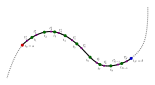
\includegraphics[width = \textwidth]{arc_length}
\end{center}

The length \(L\) of the curve between the points where \(t = a\) and \(b\) can be approximated adding the distances between consecutive pairs of points:
\[L\Big|_a^b = \|\mathbf{q}(t_1) - \mathbf{q}(t_0)\| + \|\mathbf{q}(t_2) - \mathbf{q}(t_1)\| + ... + \|\mathbf{q}(t_N) - \mathbf{q}(t_{N-1})\| = \sum_{i=1}^N \|\mathbf{q}(t_i) - \mathbf{q}(t_{i-1})\|\]

For each \(i = 1, 2, ..., N\), the distance between point \(i-1\) and point \(i\) can be approximated by the product of the speed and the change in the time \(t\): 
\[\|\mathbf{q}(t_i) - \mathbf{q}(t_{i-1})\| 
\approx \left\|\left.\frac{d\mathbf{q}}{dt}\right|_{t_i^*}(t_i - t_{i-1})\right\| 
= \left\|\left.\frac{d\mathbf{q}}{dt}\right|_{t_i^*}\Delta t_i\right\|
= \left\|\left.\frac{d\mathbf{q}}{dt}\right|_{t_i^*}\right\|\Delta t_i\]

The length is: 
\begin{align*}
L\Big|_a^b = & \lim_{N \to +\infty} \sum_{i=1}^N \|\mathbf{q}(t_i) - \mathbf{q}(t_{i-1})\| 
= \lim_{N \to +\infty} \sum_{i=1}^N \left\|\left.\frac{d\mathbf{q}}{dt}\right|_{t_i^*}\right\|\Delta t_i 
\end{align*}
The Riemannian sum evaluates the integral:
\[L\Big|_a^b = \int_{t = a}^b \left\|\frac{d\mathbf{q}}{dt}\right\| dt\]

In essence, the arc-length is the integral of the speed over the time interval.

It should also be noted that if \(b < a\), then the arc-length will be negative. Rolling \(t\) backwards results in negative distances. Flipping the bounds of a definite integral flips its sign. 

\vspace{5mm}

\textbf{Example:}
\begin{itemize}
%%%%%%%%%%%%%%%%%%%%%%%%%%%%%%%%%%%%%
\item Consider the parametric curve:
\[C: \left\{\begin{array}{c} 
x(t) = 5 \cos t \\  
y(t) = 5 \sin t \\ 
z(t) = 3t 
\end{array}\right.\]
This curve is a helix. The arc length from \(t = 0\) to \(t = 2\pi\) is sought.
\[\mathbf{q}(t) = \begin{bmatrix}
5 \cos t \\  
5 \sin t \\ 
3t 
\end{bmatrix} \quad\quad\text{and}\quad\quad \frac{d\mathbf{q}}{dt} = \begin{bmatrix}
-5 \sin t \\  
5 \cos t \\ 
3  
\end{bmatrix}\]
The speed is:
\[\left\|\frac{d\mathbf{q}}{dt}\right\| = \sqrt{25\sin^2 t + 25\cos^2 t + 9} = \sqrt{34}\] 
The arc length from \(t = 0\) to \(t = 2\pi\) is: 
\begin{align*}
L\Big|_0^{2\pi} = & \int_{t = 0}^{2\pi} \left\|\frac{d\mathbf{q}}{dt}\right\|dt 
= \int_{t = 0}^{2\pi} \sqrt{34} \cdot dt 
= \sqrt{34} \cdot t \bigg|_{t = 0}^{2\pi}   
= 2\pi\sqrt{34}
\end{align*} 
\end{itemize}




\subsection*{The arc length parameterization}  

Often, the value of \(t\) that indexes each point on a parametric curve is not of interest. What is of interest is the shape of the curve itself. The {\bf arc-length parameterization} of a curve is a parameterization where the parameter \(s\) does not represent ``time", but instead is the distance along the curve from some initial point \(\mathbf{q}(0) = \mathbf{q}_0\). The point \(\mathbf{q}_s(s)\) (note the subscript of \(s\) on \(\mathbf{q}_s\)) that is generated by a parameter value of \(s\) is the point that is a distance of \(s\) from \(\mathbf{q}_0\) along the curve. The initial parameterization \(\mathbf{q}(t)\) places an ``orientation", or in other words a ``preferred direction", on the curve. Values of \(t\) that are negative correspond to negative values of \(s\). \(t = 0\) corresponds to \(s = 0\), and values of \(t\) that are positive correspond to positive values of \(s\). In the image below, the arc-length parameterization is illustrated by spacing the points where \(s = ..., -5, -4, -3, -2, -1, 0, 1, 2, 3, 4, 5, ...\) evenly along the depicted curve. Note that while the original parameter \(t\) increases with \(s\), and \(t = 0\) when \(s = 0\), \(t\) is not equal to \(s\).   

\begin{center}
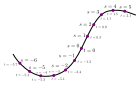
\includegraphics[width = \textwidth]{arc_length_parameterization}
\end{center}

How can an arc-length parameterization be derived from the initial parameterization \(\mathbf{q}(t)\)? Firstly, a general expression that computes the arc length \(L\Big|_{t = 0}^{t = t_{\text{curr}}}\) between \(t = 0\) and \(t = t_{\text{curr}}\) needs to be determined. \(t_{\text{curr}}\) is the value of \(t\) at the point where \(s\) is {\bf curr}ently being computed. The subscript ``curr" distinguishes this quantity from the variable of integration \(t\). The value of the parameter \(s\) at the point where \(t = t_{\text{curr}}\) is this arc-length: \(s = L\Big|_{t = 0}^{t = t_{\text{curr}}}\). Next, an expression that computes the value of \(t_{\text{curr}}\) given an arbitrary arc-length \(s\) needs to be solved for. With \(t_{\text{curr}}\) as an expression of \(s\), the point generated by \(s\), \(\mathbf{q}_s(s)\), is the point that is generated by \(t = t_{\text{curr}}\) in the original parameterization. See the following examples for more details:

\vspace{5mm}

\textbf{Examples:}
\begin{itemize}
%%%%%%%%%%%%%%%%%%%%%%%%%%%%%%%%%%%%%%%
\item Consider the parametric curve:
\[C: \left\{\begin{array}{c} 
x(t) = 5 \cos t \\  
y(t) = 5 \sin t \\ 
z(t) = 3t 
\end{array}\right.\]
This curve is a helix. To find an arc-length parameterization of this helix, \(t_{\text{curr}}\) will be arbitrary and the arc-length from \(t = 0\) to \(t = t_{\text{curr}}\) will be computed:
\[\mathbf{q}(t) = \begin{bmatrix}
5 \cos t \\  
5 \sin t \\ 
3t 
\end{bmatrix} \quad\quad\text{and}\quad\quad \frac{d\mathbf{q}}{dt} = \begin{bmatrix}
-5 \sin t \\  
5 \cos t \\ 
3  
\end{bmatrix}\]
The speed is:
\[\left\|\frac{d\mathbf{q}}{dt}\right\| = \sqrt{25\sin^2 t + 25\cos^2 t + 9} = \sqrt{34}\] 
The arc length \(s\) from \(t = 0\) to \(t = t_{\text{curr}}\) is: 
\begin{align*}
s = L\Big|_0^{t_{\text{curr}}} = & \int_{t = 0}^{t_{\text{curr}}} \left\|\frac{d\mathbf{q}}{dt}\right\|dt 
= \int_{t = 0}^{t_{\text{curr}}} \sqrt{34} \cdot dt 
= \sqrt{34} \cdot t \bigg|_{t = 0}^{t_{\text{curr}}}  
= \sqrt{34} \cdot t_{\text{curr}}
\end{align*} 
The value of \(t_{\text{curr}}\) that results in an arbitrary arc-length of \(s\) is found by solving for \(t_{\text{curr}}\):
\[s = \sqrt{34} \cdot t_{\text{curr}} \iff t_{\text{curr}} = \frac{s}{\sqrt{34}}\]  
The point generated by an arbitrary value of \(s\) is the point that is generated by the original parameterization with \(t = t_{\text{curr}} = \frac{s}{\sqrt{34}}\):
\[\mathbf{q}_s(s) = \mathbf{q}\left(\frac{s}{\sqrt{34}}\right) = \begin{bmatrix}  
5 \cos(s/\sqrt{34}) \\  
5 \sin(s/\sqrt{34}) \\ 
(3/\sqrt{34})s 
\end{bmatrix}\]
\(t = \frac{s}{\sqrt{34}}\) or equivalently \(s = \sqrt{34} \cdot t\) is the relationship between the parameters \(t\) and \(s\) at each point on the curve.
\end{itemize}

\vspace{5mm}

It is at this point worth mentioning that given an arbitrary quantity \(f\), scalar or vector valued, that varies with different points along the curve, that the chain rule gives: 
\[\frac{df}{dt} = \frac{ds}{dt}\frac{df}{ds} = \left\|\frac{d\mathbf{q}}{dt}\right\|\frac{df}{ds}\]
In other words, the rate at which \(f\) changes with respect to time, \(\frac{df}{dt}\), is equal to the rate at which \(f\) changes with respect to distance, \(\frac{df}{ds}\), multiplied by the speed \(\left\|\frac{d\mathbf{q}}{dt}\right\|\): 
\[\frac{df}{dt} = \left\|\frac{d\mathbf{q}}{dt}\right\|\frac{df}{ds} \quad\quad\text{or equivalently}\quad\quad \frac{df}{ds} = \frac{df/dt}{\|d\mathbf{q}/dt\|}\]




\subsection*{Tangent vectors}

Given a parametric curve \(\mathbf{q}(t)\) and an arbitrary point at \(t = t_0\), a line that is tangent to the curve at the point \(\mathbf{q}(t_0)\) is parallel to the velocity vector \(\left.\frac{d\mathbf{q}}{dt}\right|_{t_0}\). Parametric equations for this line are:
\[\mathbf{q}_L(u) = \mathbf{q}(t_0) + u \cdot \left.\frac{d\mathbf{q}}{dt}\right|_{t_0}\]

\begin{center}
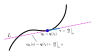
\includegraphics[width = \textwidth]{parametric_curve_tangents}
\end{center}

\textbf{Example:}
\begin{itemize}
\item Consider the parametric curve:
\[C: \left\{\begin{array}{c} 
x(t) = 5 \cos t \\  
y(t) = 5 \sin t \\ 
z(t) = 3t 
\end{array}\right.\]
This curve is a helix. Parametric equations of the tangent line that passes through the point where \(t = \pi/2\) is sought.
\[\mathbf{q}(t) = \begin{bmatrix}
5 \cos t \\  
5 \sin t \\ 
3t 
\end{bmatrix} \quad\quad\text{and}\quad\quad \frac{d\mathbf{q}}{dt} = \begin{bmatrix}
-5 \sin t \\  
5 \cos t \\ 
3  
\end{bmatrix}\]
The point on the helix where the tangent is being computed is: \(\mathbf{q}_0 = \mathbf{q}(\pi/2) = \begin{bmatrix} 0 \\ 5 \\ 3\pi/2 \end{bmatrix}\). The tangent line is parallel to \(\mathbf{v} = \left.\frac{d\mathbf{q}}{dt}\right|_{\pi/2} = \begin{bmatrix} -5 \\ 0 \\ 3 \end{bmatrix}\). Parametric equations for the tangent line are:
\[\mathbf{q}_L(u) = \begin{bmatrix} 0 \\ 5 \\ 3\pi/2 \end{bmatrix} + u \begin{bmatrix} -5 \\ 0 \\ 3 \end{bmatrix} = \begin{bmatrix} -5u \\ 5 \\ 3\pi/2 + 3u \end{bmatrix}\]
\end{itemize}

\vspace{5mm} 

The {\bf unit length tangent vector} \(\mathbf{T}\) is a unit length vector that is tangent to the curve at the current point. The unit length tangent vector is the velocity divided by the speed:
\[\mathbf{T} = \frac{d\mathbf{q}/dt}{\|d\mathbf{q}/dt\|}\]
Moreover, the unit length tangent vector is also the rate of change of the position \(\mathbf{q}\) with respect to distance \(s\) as opposed to time \(t\). \(\frac{d\mathbf{q}}{ds} = \frac{d\mathbf{q}/dt}{\|d\mathbf{q}/dt\|}\) due to the relationship between rates of change with respect to \(t\) and \(s\) discussed previously. Therefore:
\[\mathbf{T} = \frac{d\mathbf{q}/dt}{\|d\mathbf{q}/dt\|} \quad\quad\text{and}\quad\quad \mathbf{T} = \frac{d\mathbf{q}}{ds}\] 

\textbf{Examples:}
\begin{itemize}
%%%%%%%%%%%%%%%%%%%%%%%%%%%%%%%%%%%%%%%
\item Consider the parametric curve:
\[C: \left\{\begin{array}{c} 
x(t) = 5 \cos t \\  
y(t) = 5 \sin t \\ 
z(t) = 3t 
\end{array}\right.\]
It has already been established in previous examples that
\[\mathbf{q}(t) = \begin{bmatrix}
5 \cos t \\  
5 \sin t \\ 
3t 
\end{bmatrix} \quad\quad\text{and}\quad\quad \frac{d\mathbf{q}}{dt} = \begin{bmatrix}
-5 \sin t \\  
5 \cos t \\ 
3  
\end{bmatrix} \quad\quad\text{and}\quad\quad \left\|\frac{d\mathbf{q}}{dt}\right\| = \sqrt{34}\] 
The arc length parameter \(s\) is related to the original parameter \(t\) at each point via the relationship \(s = \sqrt{34} \cdot t\), and the arc-length parameterization itself is:
\[\mathbf{q}_s(s) = \begin{bmatrix}  
5 \cos(s/\sqrt{34}) \\  
5 \sin(s/\sqrt{34}) \\ 
(3/\sqrt{34})s 
\end{bmatrix}\] 
The unit length tangent vector can be computed by either: 
\[\mathbf{T}(t) = \frac{d\mathbf{q}/dt}{\|d\mathbf{q}/dt\|} = \begin{bmatrix}
-(5/\sqrt{34}) \sin t \\  
(5/\sqrt{34}) \cos t \\ 
3/\sqrt{34}  
\end{bmatrix}\]
or by: 
\[\mathbf{T}(s) = \frac{d\mathbf{q}_s}{ds} = \begin{bmatrix}  
-(5/\sqrt{34}) \sin(s/\sqrt{34}) \\  
(5/\sqrt{34}) \cos(s/\sqrt{34}) \\ 
3/\sqrt{34} 
\end{bmatrix}\]
these two expressions are equivalent when the fact that \(s = \sqrt{34} \cdot t\) is accounted for.
\end{itemize}





\subsection*{Normal vectors}

\begin{tabular}{cc}
\parbox{0.5\textwidth}{ 
In addition to the unit length tangent vectors, the {\bf principal unit length normal vector} \(\mathbf{N}\) is a unit vector that is perpendicular to \(\mathbf{T}\) and points in the direction that the curve is ``turning". More specifically, the rate of change of the unit length tangent vector with {\bf respect to distance} is:
\[\frac{d\mathbf{T}}{ds} = \kappa \cdot \mathbf{N}\] 
\(\kappa\), referred to as the {\bf curvature} is the magnitude of \(\frac{d\mathbf{T}}{ds}\), while the unit length normal vector \(\mathbf{N}\) is the direction of \(\frac{d\mathbf{T}}{ds}\). 

It should be noted that since the unit length tangent vector has a fixed magnitude of \(1\), the rate of change in \(\mathbf{T}\) will always be perpendicular to \(\mathbf{T}\), hence why \(\mathbf{N}\) is always perpendicular to \(\mathbf{T}\).
} & \parbox{0.5\textwidth}{
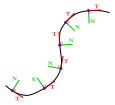
\includegraphics[width = 0.5\textwidth]{unit_tangents_and_unit_normals}
}
\end{tabular}

Consider for example a circle with an arbitrary radius of \(R\) with the parameterization:
\[\mathbf{q}(t) = \begin{bmatrix} R \cos t \\ R \sin t \\ 0 \end{bmatrix}\]  
\[\frac{d\mathbf{q}}{dt} = \begin{bmatrix} -R \sin t \\ R \cos t \\ 0 \end{bmatrix} \quad\quad\text{and}\quad\quad \left\|\frac{d\mathbf{q}}{dt}\right\| = R \quad\quad\text{and the arc-length parameter \(s\) satisfies: } s = R \cdot t\]
The arc-length parameterization itself is: 
\[\mathbf{q}_s(s) = \begin{bmatrix} R \cos(s/R) \\ R \sin(s/R) \\ 0 \end{bmatrix}\]
The unit-length tangent vector is:
\[\mathbf{T}(s) = \frac{d\mathbf{q}_s}{ds} = \begin{bmatrix} -\sin(s/R) \\ \cos(s/R) \\ 0 \end{bmatrix}\]
The rate of change of the unit length tangent vector with respect to \(s\) is:
\[\frac{d\mathbf{T}}{ds} = \begin{bmatrix} -(1/R)\cos(s/R) \\ -(1/R)\sin(s/R) \\ 0 \end{bmatrix}\]
The curvature is:
\[\kappa(s) = \left\|\frac{d\mathbf{T}}{ds}\right\| = \frac{1}{R}\]
while the principal unit length normal vector is:
\[\mathbf{N}(s) = \frac{d\mathbf{T}/ds}{\kappa} = \begin{bmatrix} -\cos(s/R) \\ -\sin(s/R) \\ 0 \end{bmatrix}\]
\begin{tabular}{cc}
\parbox{0.4\textwidth}{
Note that from the relationship \(\kappa = \frac{1}{R}\), the {\bf radius of curvature} is \(R = \frac{1}{\kappa}\). The radius of curvature when computed at a specific point on an arbitrary curve is the radius of a circle that ``best fits" the current bend, as depicted on the right. 
} & \parbox{0.6\textwidth}{
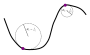
\includegraphics[width = 0.6\textwidth]{radius_of_curvature}
}
\end{tabular}


In many cases, the arc length parameterization is not easy to determine, such as in the example below: 

Consider an ellipse that is centered on the origin and has an \(x\)-radius of \(a\) and a \(y\)-radius of \(b\). A parameterization of this ellipse is:
\[\mathbf{q}(t) = \begin{bmatrix} a \cos t \\ b \sin t \\ 0 \end{bmatrix}\]  
\[\frac{d\mathbf{q}}{dt} = \begin{bmatrix} -a \sin t \\ b \cos t \\ 0 \end{bmatrix} \quad\quad\text{and}\quad\quad \left\|\frac{d\mathbf{q}}{dt}\right\| = \sqrt{a^2\sin^2 t + b^2 \cos^2 t}\] 

The value of the arc-length \(s\) when \(t = t_{\text{curr}}\) is given by the integral:
\[s = \int_{t = 0}^{t_{\text{curr}}} \sqrt{a^2\sin^2 t + b^2 \cos^2 t} \cdot dt\]
There is no easy solution to this integral. Despite this however, the curvature and unit normal vectors can still be computed. Two approaches will be described:




\subsubsection*{Converting rates of change}

While expressing quantities in terms of the arc-length \(s\) may be difficult, the rate of change with respect to the arc-length can be easily determined from the rate of change with respect to time by dividing by the speed. Therefore \(\frac{d\mathbf{T}}{ds}\) can be computed from \(\frac{d\mathbf{T}}{dt}\) via:

\[\frac{d\mathbf{T}}{ds} = \frac{d\mathbf{T}/dt}{\|d\mathbf{q}/dt\|}\]

The curvature and principal unit normal vector are:

\[\kappa = \left\|\frac{d\mathbf{T}}{ds}\right\| = \frac{\left\|d\mathbf{T}/dt\right\|}{\|d\mathbf{q}/dt\|}\] 
and
\[\mathbf{N} = \frac{d\mathbf{T}/ds}{\kappa} = \frac{d\mathbf{T}/dt}{\|d\mathbf{T}/dt\|}\]

Returning to the ellipse example, 

\[\mathbf{q}(t) = \begin{bmatrix} a \cos t \\ b \sin t \\ 0 \end{bmatrix} \quad\quad\text{and}\quad\quad \frac{d\mathbf{q}}{dt} = \begin{bmatrix} -a \sin t \\ b \cos t \\ 0 \end{bmatrix} \quad\quad\text{and}\quad\quad \left\|\frac{d\mathbf{q}}{dt}\right\| = \sqrt{a^2\sin^2 t + b^2 \cos^2 t}\]

The unit length tangent vector is:
\[\mathbf{T}(t) = \frac{d\mathbf{q}/dt}{\|d\mathbf{q}/dt\|} = \begin{bmatrix} -a\sin t / \sqrt{a^2\sin^2 t + b^2 \cos^2 t} \\ b\cos t / \sqrt{a^2\sin^2 t + b^2 \cos^2 t} \\ 0 \end{bmatrix}\]

Differentiating with respect to \(t\) gives:

\begin{align*}
\frac{d\mathbf{T}}{dt} = & \frac{-ab}{(a^2\sin^2 t + b^2 \cos^2 t)^{3/2}}\begin{bmatrix} 
b\cos t \\ 
a \sin t \\ 
0 \end{bmatrix}
\end{align*}

Next:
\[\left\|\frac{d\mathbf{T}}{dt}\right\| = \frac{ab}{a^2\sin^2 t + b^2 \cos^2 t}\]

Lastly, 

\[\kappa(t) = \frac{\|d\mathbf{T}/dt\|}{\|d\mathbf{q}/dt\|} = \frac{ab}{(a^2\sin^2 t + b^2 \cos^2 t)^{3/2}}\]

and 

\[\mathbf{N}(t) = \frac{d\mathbf{T}/dt}{\|d\mathbf{T}/dt\|} = \begin{bmatrix} -b\cos t /\sqrt{a^2\sin^2 t + b^2 \cos^2 t} \\ -a\sin t / \sqrt{a^2\sin^2 t + b^2 \cos^2 t} \\ 0 \end{bmatrix}\]




\subsubsection*{Using the acceleration}

The curvature and principal unit normal vectors can also be derived by observing that the velocity \(\frac{d\mathbf{q}}{dt}\) is a multiple of \(\mathbf{T}\), and that the acceleration \(\frac{d^2\mathbf{q}}{dt^2}\) is a linear combination of both \(\mathbf{T}\) and \(\mathbf{N}\).  

To simplify matters, the speed will be denoted by \(V\): \(V = \left\|\frac{d\mathbf{q}}{dt}\right\|\).  

It is clear from the definition of \(V\) and \(\mathbf{T}\) that the velocity can be expressed as:
\[\frac{d\mathbf{q}}{dt} = V \cdot \mathbf{T}\]
computing the acceleration using the product rule gives:
\begin{align*}
\frac{d^2 \mathbf{q}}{dt^2} = & \frac{d}{dt}(V \cdot \mathbf{T}) 
= \frac{dV}{dt} \cdot \mathbf{T} + V \cdot \frac{d\mathbf{T}}{dt}
\end{align*}
The relationship between rates of change with respect to \(t\) and rates of change with respect to \(s\) yields: 
\[\frac{d\mathbf{T}}{dt} = \left\|\frac{d\mathbf{q}}{dt}\right\| \frac{d\mathbf{T}}{ds} = V \frac{d\mathbf{T}}{ds}\]
This, together with the definition:
\[\frac{d\mathbf{T}}{ds} = \kappa \cdot \mathbf{N}\]
gives: 
\begin{align*}
\frac{d^2 \mathbf{q}}{dt^2} = & \frac{dV}{dt} \cdot \mathbf{T} + V^2 \cdot \kappa \cdot \mathbf{N}
\end{align*}
\begin{center}
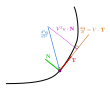
\includegraphics[width = 0.75\textwidth]{acceleration_perpendicular_component}
\end{center}
The component of the acceleration \(\frac{d^2 \mathbf{q}}{dt^2}\) that is perpendicular to \(\mathbf{T}\), and hence perpendicular to the velocity \(\frac{d\mathbf{q}}{dt}\), has a magnitude of \(V^2 \cdot \kappa\). The magnitude of the component of \(\frac{d^2 \mathbf{q}}{dt^2}\) that is perpendicular to \(\frac{d\mathbf{q}}{dt}\) is also computed by the formula:
\[\left\|\text{perp}\left(\frac{d^2 \mathbf{q}}{dt^2}\middle|\frac{d\mathbf{q}}{dt}\right)\right\| = \frac{\left\|\frac{d\mathbf{q}}{dt} \times \frac{d^2 \mathbf{q}}{dt^2}\right\|}{\left\|\frac{d\mathbf{q}}{dt}\right\|}\]
The magnitude is known to be \(V^2 \cdot \kappa\), so therefore:
\begin{align*}
& \left\|\text{perp}\left(\frac{d^2 \mathbf{q}}{dt^2}\middle|\frac{d\mathbf{q}}{dt}\right)\right\| = V^2 \cdot \kappa 
\iff V^2 \cdot \kappa = \frac{\left\|\frac{d\mathbf{q}}{dt} \times \frac{d^2 \mathbf{q}}{dt^2}\right\|}{\left\|\frac{d\mathbf{q}}{dt}\right\|} 
\iff \kappa = \frac{\left\|\frac{d\mathbf{q}}{dt} \times \frac{d^2 \mathbf{q}}{dt^2}\right\|}{V^2 \left\|\frac{d\mathbf{q}}{dt}\right\|} = \frac{\left\|\frac{d\mathbf{q}}{dt} \times \frac{d^2 \mathbf{q}}{dt^2}\right\|}{\left\|\frac{d\mathbf{q}}{dt}\right\|^3}
\end{align*}
The curvature \(\kappa\) is therefore
\[\kappa(t) = \frac{\left\|\frac{d\mathbf{q}}{dt} \times \frac{d^2 \mathbf{q}}{dt^2}\right\|}{\left\|\frac{d\mathbf{q}}{dt}\right\|^3}\]
The unit length normal vector \(\mathbf{N}\) can then be computed by dividing the perpendicular component \(\text{perp}\left(\frac{d^2 \mathbf{q}}{dt^2}\middle|\frac{d\mathbf{q}}{dt}\right)\) by its known magnitude \(V^2 \cdot \kappa = \frac{\left\|\frac{d\mathbf{q}}{dt} \times \frac{d^2 \mathbf{q}}{dt^2}\right\|}{\left\|\frac{d\mathbf{q}}{dt}\right\|}\):
\[\mathbf{N}(t) = \frac{\left\|\frac{d\mathbf{q}}{dt}\right\|}{\left\|\frac{d\mathbf{q}}{dt} \times \frac{d^2 \mathbf{q}}{dt^2}\right\|}\text{perp}\left(\frac{d^2 \mathbf{q}}{dt^2}\middle|\frac{d\mathbf{q}}{dt}\right)\]



Return now to the ellipse example:
\[\mathbf{q}(t) = \begin{bmatrix} a \cos t \\ b \sin t \\ 0 \end{bmatrix} \quad\quad\text{and}\quad\quad \frac{d\mathbf{q}}{dt} = \begin{bmatrix} -a \sin t \\ b \cos t \\ 0 \end{bmatrix} \quad\quad\text{and}\quad\quad \left\|\frac{d\mathbf{q}}{dt}\right\| = \sqrt{a^2\sin^2 t + b^2 \cos^2 t}\]
\[\quad\quad\text{and}\quad\quad \frac{d^2\mathbf{q}}{dt^2} = \begin{bmatrix} -a \cos t \\ -b \sin t \\ 0 \end{bmatrix}\]

The cross-product of the velocity and acceleration is:
\[\frac{d\mathbf{q}}{dt} \times \frac{d^2\mathbf{q}}{dt^2} = \begin{bmatrix} -a \sin t \\ b \cos t \\ 0 \end{bmatrix} \times \begin{bmatrix} -a \cos t \\ -b \sin t \\ 0 \end{bmatrix} 
= \begin{bmatrix} 0 - 0 \\ 0 - 0 \\ ab\sin^2 t - (-ab\cos^2 t) \end{bmatrix} = \begin{bmatrix} 0 \\ 0 \\ ab \end{bmatrix}\]
so 
\[\left\|\frac{d\mathbf{q}}{dt} \times \frac{d^2\mathbf{q}}{dt^2}\right\| = ab\]
The curvature as a function of \(t\) is therefore:
\[\kappa(t) = \frac{ab}{(a^2\sin^2 t + b^2 \cos^2 t)^{3/2}}\] 

Now to compute the unit normal vectors. Firstly compute the component of the acceleration that is perpendicular to the velocity: 
\begin{align*}
& \text{perp}\left(\frac{d^2 \mathbf{q}}{dt^2}\middle|\frac{d\mathbf{q}}{dt}\right) 
= \frac{d^2 \mathbf{q}}{dt^2} - \text{proj}\left(\frac{d^2 \mathbf{q}}{dt^2}\middle|\frac{d\mathbf{q}}{dt}\right) 
= \frac{d^2 \mathbf{q}}{dt^2} - \frac{\frac{d\mathbf{q}}{dt} \bullet \frac{d^2 \mathbf{q}}{dt^2}}{\left\|\frac{d\mathbf{q}}{dt}\right\|^2}\frac{d\mathbf{q}}{dt} \\
& = \begin{bmatrix} -a \cos t \\ -b \sin t \\ 0 \end{bmatrix} - \frac{(a^2 - b^2) \cos t \sin t}{a^2\sin^2 t + b^2 \cos^2 t}\begin{bmatrix} -a \sin t \\ b \cos t \\ 0 \end{bmatrix} \\
& = \frac{1}{a^2\sin^2 t + b^2 \cos^2 t}\begin{bmatrix} 
(-ab^2 \cos^3 t - a^3 \cos t \sin^2 t) + (a^3 - ab^2)\cos t \sin^2 t \\  
(-b^3 \cos^2 t \sin t - a^2 b \sin^3 t) + (-a^2b + b^3)\cos^2 t \sin t \\
0 \end{bmatrix} \\  
& = \frac{1}{a^2\sin^2 t + b^2 \cos^2 t}\begin{bmatrix} 
-ab^2 \cos^3 t - ab^2 \cos t \sin^2 t \\  
-a^2 b \sin^3 t - a^2b \cos^2 t \sin t \\
0 \end{bmatrix}  
= \frac{1}{a^2\sin^2 t + b^2 \cos^2 t}\begin{bmatrix} 
-ab^2 \cos t \\  
-a^2 b \sin t \\
0 \end{bmatrix}
\end{align*}
The unit length normals are now:
\begin{align*}
\mathbf{N}(t) = & \frac{\left\|\frac{d\mathbf{q}}{dt}\right\|}{\left\|\frac{d\mathbf{q}}{dt} \times \frac{d^2 \mathbf{q}}{dt^2}\right\|}\text{perp}\left(\frac{d^2 \mathbf{q}}{dt^2}\middle|\frac{d\mathbf{q}}{dt}\right) 
= \frac{\sqrt{a^2\sin^2 t + b^2 \cos^2 t}}{ab} \cdot \frac{1}{a^2\sin^2 t + b^2 \cos^2 t}\begin{bmatrix} 
-ab^2 \cos t \\  
-a^2 b \sin t \\
0 \end{bmatrix} \\
= & \frac{1}{\sqrt{a^2\sin^2 t + b^2 \cos^2 t}}\begin{bmatrix} -b\cos t \\ -a \sin t \\ 0 \end{bmatrix}  
\end{align*}

%\subsection*{Binormal vectors}



\subsubsection*{Three approaches}

In summary there are 3 approaches to finding the unit length tangent and the principal unit normal vectors, as well as the curvature. This will be illustrated using the same helix 
\[\mathbf{q}(t) = \begin{bmatrix} 
5 \cos t \\  
5 \sin t \\ 
3t 
\end{bmatrix}\]  
the velocity and speed are respectively:
\[\frac{d\mathbf{q}}{dt} = \begin{bmatrix} 
-5 \sin t \\  
5 \cos t \\ 
3 
\end{bmatrix}
\quad\quad\text{and}\quad\quad
\left\|\frac{d\mathbf{q}}{dt}\right\| = \sqrt{34}\]


\textbf{Approach \#1: Using the arc length parameterization:}

The arc length is related to time via \(s = \sqrt{34} \cdot t\), so the arc length parameterization is:
\[\mathbf{q}_s(s) = \begin{bmatrix} 
5 \cos (s/\sqrt{34}) \\  
5 \sin (s/\sqrt{34}) \\ 
(3/\sqrt{34})s 
\end{bmatrix}\] 

The unit length tangent vectors are: 
\[\mathbf{T}(s) = \frac{d\mathbf{q}_s}{ds} = \begin{bmatrix} -(5/\sqrt{34})\sin(s/\sqrt{34}) \\ (5/\sqrt{34})\cos(s/\sqrt{34}) \\ 3/\sqrt{34} \end{bmatrix}\]

Differentiating with respect to \(s\) gives:
\[\frac{d\mathbf{T}}{ds} = \begin{bmatrix} -(5/34)\cos(s/\sqrt{34}) \\ -(5/34)\sin(s/\sqrt{34}) \\ 0 \end{bmatrix}\] 

so the curvature and principal unit normal vectors are:

\[\kappa(s) = \left\|\frac{d\mathbf{T}}{ds}\right\| = \frac{5}{34}
\quad\quad\text{and}\quad\quad
\mathbf{N}(s) = \frac{d\mathbf{T}/ds}{\kappa(s)} = \begin{bmatrix} -\cos(s/\sqrt{34}) \\ -\sin(s/\sqrt{34}) \\ 0 \end{bmatrix}\]


\textbf{Approach \#2: Converting the rates of change}

Often, the arc length parameterization cannot be derived. In this case, the rates of change with respect to time can be converted to rates of change with respect to arc length. 

The unit length tangent vectors are: 
\[\mathbf{T}(t) = \frac{d\mathbf{q}/dt}{\|d\mathbf{q}/dt\|} = \frac{1}{\sqrt{34}}\begin{bmatrix} -5 \sin t \\ 5 \cos t \\ 3 \end{bmatrix} = \begin{bmatrix} -(5/\sqrt{34})\sin t \\ (5/\sqrt{34})\cos t \\ 3/\sqrt{34} \end{bmatrix}\]  

Differentiating with respect to \(t\) gives:
\[\frac{d\mathbf{T}}{dt} = \begin{bmatrix} -(5/\sqrt{34})\cos t \\ -(5/\sqrt{34})\sin t \\ 0 \end{bmatrix}\]

Next:
\[\left\|\frac{d\mathbf{T}}{dt}\right\| = \frac{5}{\sqrt{34}}\]

Lastly,
\[\kappa(t) = \frac{\|d\mathbf{T}/dt\|}{\|d\mathbf{q}/dt\|} = \frac{5}{34}
\quad\quad\text{and}\quad\quad
\mathbf{N}(t) = \frac{d\mathbf{T}/dt}{\|d\mathbf{T}/dt\|} = \begin{bmatrix} -\cos t \\ -\sin t \\ 0 \end{bmatrix}\]


\textbf{Approach \#3: Using the acceleration}

The unit length tangent vectors are: 
\[\mathbf{T}(t) = \frac{d\mathbf{q}/dt}{\|d\mathbf{q}/dt\|} = \frac{1}{\sqrt{34}}\begin{bmatrix} -5 \sin t \\ 5 \cos t \\ 3 \end{bmatrix} = \begin{bmatrix} -(5/\sqrt{34})\sin t \\ (5/\sqrt{34})\cos t \\ 3/\sqrt{34} \end{bmatrix}\]  

The acceleration is:
\[\frac{d^2 \mathbf{q}}{dt^2} = \begin{bmatrix} -5 \cos t \\ -5 \sin t \\ 0 \end{bmatrix}\]

The cross product of the velocity and acceleration is:
\begin{align*}
\frac{d\mathbf{q}}{dt} \times \frac{d^2 \mathbf{q}}{dt^2} 
& = \begin{bmatrix} -5 \sin t \\ 5 \cos t \\ 3 \end{bmatrix} \times \begin{bmatrix} -5 \cos t \\ -5 \sin t \\ 0 \end{bmatrix}
= \begin{bmatrix} (5\cos t)(0) - (3)(-5\sin t) \\ (3)(-5\cos t) - (-5\sin t)(0) \\ (-5\sin t)(-5\sin t) - (5\cos t)(-5\cos t) \end{bmatrix} \\ 
& = \begin{bmatrix} 15\sin t \\ -15\cos t \\ 25\sin^2 t + 25\cos^2 t \end{bmatrix} 
= \begin{bmatrix} 15\sin t \\ -15\cos t \\ 25 \end{bmatrix}
\end{align*}
so
\[\left\|\frac{d\mathbf{q}}{dt} \times \frac{d^2 \mathbf{q}}{dt^2}\right\| = \sqrt{225\sin^2 t + 225\cos^2 t + 625} = \sqrt{850} = 5\sqrt{34}\]

The curvature is: 
\[\kappa(t) = \frac{\left\|\frac{d\mathbf{q}}{dt} \times \frac{d^2 \mathbf{q}}{dt^2}\right\|}{\left\|\frac{d\mathbf{q}}{dt}\right\|^3} = \frac{5\sqrt{34}}{(\sqrt{34})^3} = \frac{5}{34}\]

Now to compute the unit normal vectors. Firstly compute the component of the acceleration that is perpendicular to the velocity: 
\begin{align*}
\text{perp}\left(\frac{d^2 \mathbf{q}}{dt^2}\middle|\frac{d\mathbf{q}}{dt}\right) 
& = \frac{d^2 \mathbf{q}}{dt^2} - \text{proj}\left(\frac{d^2 \mathbf{q}}{dt^2}\middle|\frac{d\mathbf{q}}{dt}\right) 
= \frac{d^2 \mathbf{q}}{dt^2} - \frac{\frac{d\mathbf{q}}{dt} \bullet \frac{d^2 \mathbf{q}}{dt^2}}{\left\|\frac{d\mathbf{q}}{dt}\right\|^2}\frac{d\mathbf{q}}{dt} \\
& = \begin{bmatrix} -5 \cos t \\ -5 \sin t \\ 0 \end{bmatrix} - \frac{25\sin t \cos t - 25\cos t \sin t}{34}\begin{bmatrix} 
-5 \sin t \\  
5 \cos t \\ 
3 
\end{bmatrix}
= \begin{bmatrix} -5 \cos t \\ -5 \sin t \\ 0 \end{bmatrix}
\end{align*}

The unit length normals are now:
\begin{align*}
\mathbf{N}(t) 
& = \frac{\left\|\frac{d\mathbf{q}}{dt}\right\|}{\left\|\frac{d\mathbf{q}}{dt} \times \frac{d^2 \mathbf{q}}{dt^2}\right\|}\text{perp}\left(\frac{d^2 \mathbf{q}}{dt^2}\middle|\frac{d\mathbf{q}}{dt}\right) 
= \frac{\sqrt{34}}{5\sqrt{34}}\begin{bmatrix} -5 \cos t \\ -5 \sin t \\ 0 \end{bmatrix}
= \begin{bmatrix} -\cos t \\ -\sin t \\ 0 \end{bmatrix}
\end{align*}

\end{document}

















